\chapter{Control Software}

In order to control the whole automated assembly system a PC-based Qt-application was developed. All the necessary hardware is connected to the PC with USB interface.

\section{General structure of the application}

\subsection{Model View Controller architectural pattern}

The architecture of the application is based on Model-View-Controller (MVC) architectural pattern. It considers there to be three main types of objects: model objects, view objects and controller objects. When designing an application, a major step is choosing or creating custom classes for objects that fall into one of these three groups. Each of the three types of objects is separated from the others by abstract boundaries and communicates with objects of the other types across those boundaries. The pattern defines not only the roles objects play in the application, it also defines the way objects communicate with each other \cite{apple_MVC}. The key point of MVC is that View and Controller depend on Model, but Model does not depend on them. The  interaction of these three types is schematically shown in the Figure \ref{fig:mvc_general}.

\begin{figure}[ht]\centering
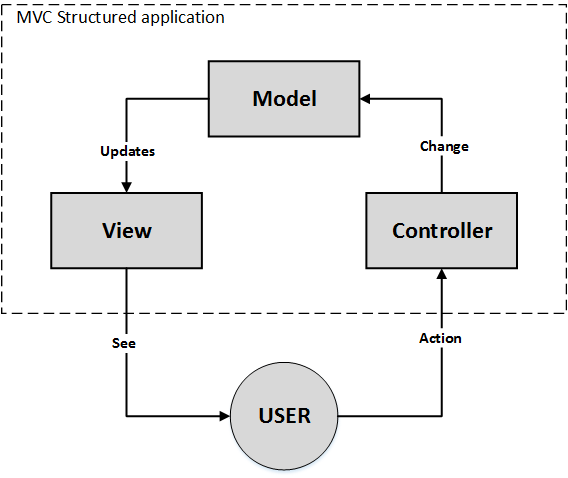
\includegraphics[width=0.7\linewidth]{Data/Control_Software/MVC_general.png}
\caption{Model, View and Controller (MVC) relative to user.}
\label{fig:mvc_general}
\end{figure}

Shown in the Figure \ref{fig:mvc_general} interaction is a classical MVC architecture. There are various realization of this diagram in terms of interaction between three main object types of MVC. The main reasons of it are various application types and their realizations. For instance, in our application this diagram will look like in the Figure \ref{fig:mvc_custom}.

\begin{figure}[ht]\centering
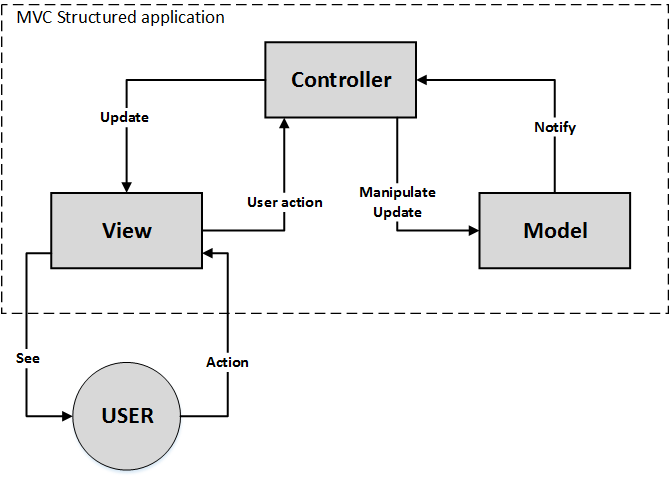
\includegraphics[width=0.7\linewidth]{Data/Control_Software/MVC_custom.png}
\caption{Model, View and Controller (MVC) relative to user.}
\label{fig:mvc_custom}
\end{figure}

Comparing to classical MVC structure from Figure \ref{fig:mvc_general}, the Model do not directly inform/update the View. This information passes through Controller. A controller object acts as the intermediary between the Model and the View. Controllers are often in charge of making sure the views have access to the model objects they need to display and act as the conduit through which views learn about changes to the model. Controller objects can also perform set-up and coordinating tasks for an application and manage the life cycles of other objects \cite{apple_MVC}.

Depending on the application logic and demands, Model, View and Controller follow special properties and rules.

\textit{Model} is central component of the system. It directly manages the data, defines the logic and rules of the application which manipulates the date. Moreover, like in our case, it regulates the interaction between the application and hardware. For instance, there is a Model class \textit{ConradModel} in our application. It is responsible for communication with a relay card for turning on and off vacuum lines. This class completely meet MVC rules as a Model object because it does not depend on any other class, while others depend on it using its possibilities for their functions.

\textit{View} unite all objects responsible for visual part of the application: windows, tabs, labels, forms, buttons, etc. They know how to display the data from the application's model and also give a user the possibility to edit the data. For instance, one task of \textit{AssemblyModuleAssembler} class is to display the information about Vacuum lines of the system, as well as control elements for it. However, it only display the control elements, but not process the user's actions.

\textit{Controller} is mainly responsible for accepting input and processing it, generating commands for the Model or the View. For instance, \textit{ConradManager} provides all necessary functions to control the vacuum lines and to get the current status of it. It is worth noting that very often there is no direct connection between the Model and the View, like it is shown in the classical MVC architecture in the Figure \ref{fig:mvc_general}. Instead of it, the Controller acts as the intermediary between the application's model objects and its view objects.

\section{Application functionality}

\subsection{Acquire image}

\subsection{Threshold tuner}

\subsection{Motion manager}

\section{OpenCV library}

A lot of algorithms needed for the application were found in the open-source library~---~OpenCV (\textit{Open Source Computer Vision}). It is a cross-platform library of programming functions mainly oriented on real-time computer vision. It was originally developed by Intel's research center in Nizhny Novgorod (Russia). Later it was supported by Willow Garage and is now maintained by Itseez. The library is free for use under the open-source BSD license~\cite{OpenCV_general}.

OpenCV was designed for computational efficiency and, as was already mentioned, with a strong focus on real-time applications. It is written in optimized C++ and can take advantage of multicore processors. There is also a possibility for further automatic optimization on Intel architecture with Intel's \textit{Integrated Performance Primitives (IPP)} libraries, which consist of low-level optimized routines in many different algorithmic areas~\cite{kaehler2016learning}.

One of the main goals of OpenCV is to provide a simple-to-use computer vision infrastructure that helps people build fairly sophisticated vision applications quickly. Its libraries one can find over 500 functions that span many areas in vision. In the list below one can see main features of the OpenCV library~\cite{Illinois_openCV}:
\begin{itemize}
\setlength\itemsep{-0.5em}
\item Image data manipulation (allocation, release, copying, setting, conversion).
\item Image and video I/O (file and camera based input, image/video file output).
\item Matrix and vector manipulation and linear algebra routines (products, solvers, eigenvalues, SVD).
\item Various dynamic data structures (lists, queues, sets, trees, graphs).
\item Basic image processing (filtering, edge detection, corner detection, sampling and interpolation, color conversion, morphological operations, histograms, image pyramids).
\item Structural analysis (connected components, contour processing, distance transform, various moments, template matching, Hough transform, polygonal approximation, line fitting, ellipse fitting, Delaunay triangulation).
\item Camera calibration (finding and tracking calibration patterns, calibration, fundamental matrix estimation, homography estimation, stereo correspondence).
\item Motion analysis (optical flow, motion segmentation, tracking).
\item Object recognition (eigen-methods, HMM).
\item Basic GUI (display image/video, keyboard and mouse handling, scroll-bars).
\item Image labeling (line, conic, polygon, text drawing).
\end{itemize}

The application of the OpenCV libraries will be described more detailed in the next section.

\section{Pattern recognition}

Pattern recognition is a crucial part of the whole automated assembly system. It provides the software with the information where all the components of the modules are situated in the space and theirs orientation. Within this information the software is able to calculate where to move each component of an assembling module.

\ldots\ldots\ldots


General idea
Pattern recognition steps:
Acquire image
Grayscale picture if not already.
Make binary (threshold)
Theta loop with (x;y) detection in each iteration
Find the best theta (lower point of the graph)
Provide (x;y;theta)
Theta range:
(-0.5:0.025:0.5)


\subsection{Pattern recognition algorithm}

OpenCV library, methods



\subsection{Threshold}



\subsection{Autofocus}






%\subsection{A Subsection}
